\documentclass[12pt]{beamer}
\usetheme{Pittsburgh}
%\setbeamertemplate{frametitle}[default][left]
% Somehow rightbound frame titles - change it?
\usepackage[utf8]{inputenc}
\usepackage[english]{babel}
\usepackage{amsmath}
\usepackage{amsfonts}
\usepackage{amssymb}
\usepackage{graphicx}
\usepackage{xcolor}
\author{Sebastian Valet, Johannes Walter}
\title{Human Capital Investments and Expectations about Career and Family}
%\setbeamercovered{transparent} 
%\setbeamertemplate{navigation symbols}{} 
%\logo{} 
%\institute{} 
%\date{} 
%\subject{} 
\begin{document}

\begin{frame}
\titlepage
\end{frame}

%\begin{frame}
%\tableofcontents
%\end{frame}

\begin{frame}{Summary I}
    \textbf{Research questions}
        \begin{itemize}
            \item What do students believe about the consequences of their education choices?
            \item How do students sort into majors?
            \item Novel: what role do family variables play in such choices?
        \end{itemize}
    \vspace{0.5cm}
    \textbf{Research design}
        \begin{itemize}
            \item Survey with undergraduate students at NYU on perceptions about consequences of educational choices
            \item Specifically: choice of a major
            \item Follow-up survey after six years
        \end{itemize}
\end{frame}

\begin{frame}{Summary II}
    \textbf{Results}
    \begin{itemize}
        \item Students believe in importance of consequences for own earnings and family life
        \item Particularly women, major choice also corresponds to different rates and timing of marriage and fertility
        \item Belief about marriage market "return" to higher earning majors
        \item Ex-ante beliefs are systematically related to educational choices and ex-post realized outcomes
    \end{itemize}
\end{frame}


% These sildes can probably go in the appendix
\begin{frame}{Current Population Characteristics I}
    \begin{itemize}
        \item Earnings, employment, and marriage data  for the US population using the 2009
        \item Not suited for causal inference; needs not reflect the student's beliefs
        \item Data from older cohort; includes not only high-ability participants
        \item But data is suited to document that career and family outcomes differ by educational choices in observational data
    \end{itemize}
\end{frame}

\begin{frame}{Current Population Characteristics II}
    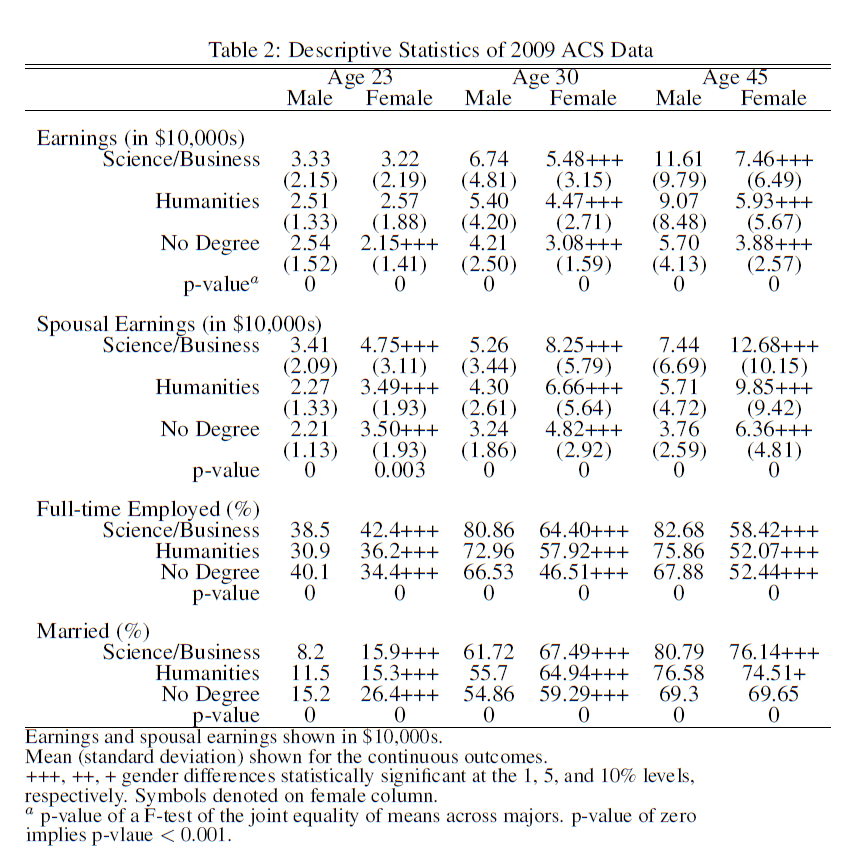
\includegraphics[scale=0.4]{Table2.png}
\end{frame}

% Earnings Beliefs: Earnings Levels
\begin{frame}{Earnings Beliefs: Earnings Levels}
    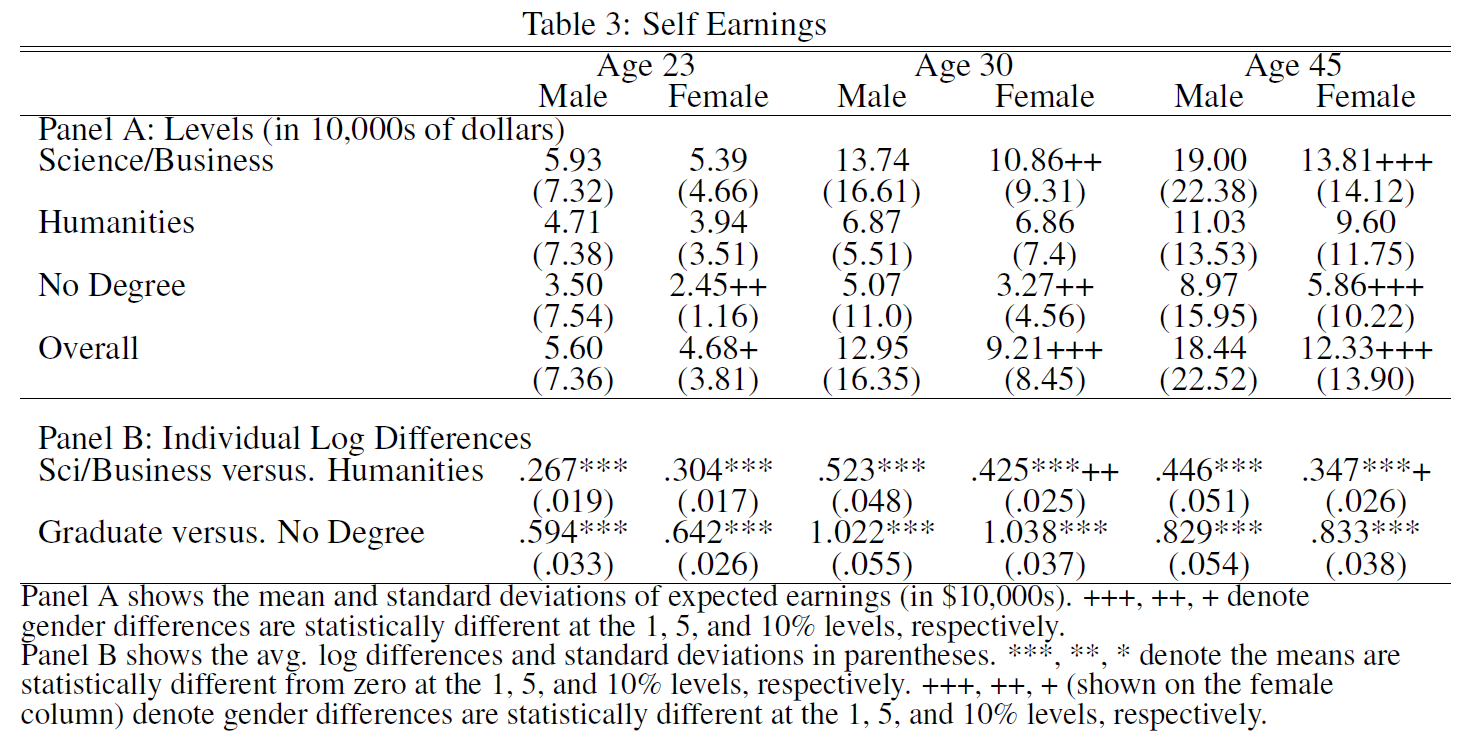
\includegraphics[scale=0.35]{Graphs/Table 3 Self Earnings.png}
\end{frame}

% Earnings Beliefs: Earnings Growth
\begin{frame}{Earnings Growth}
    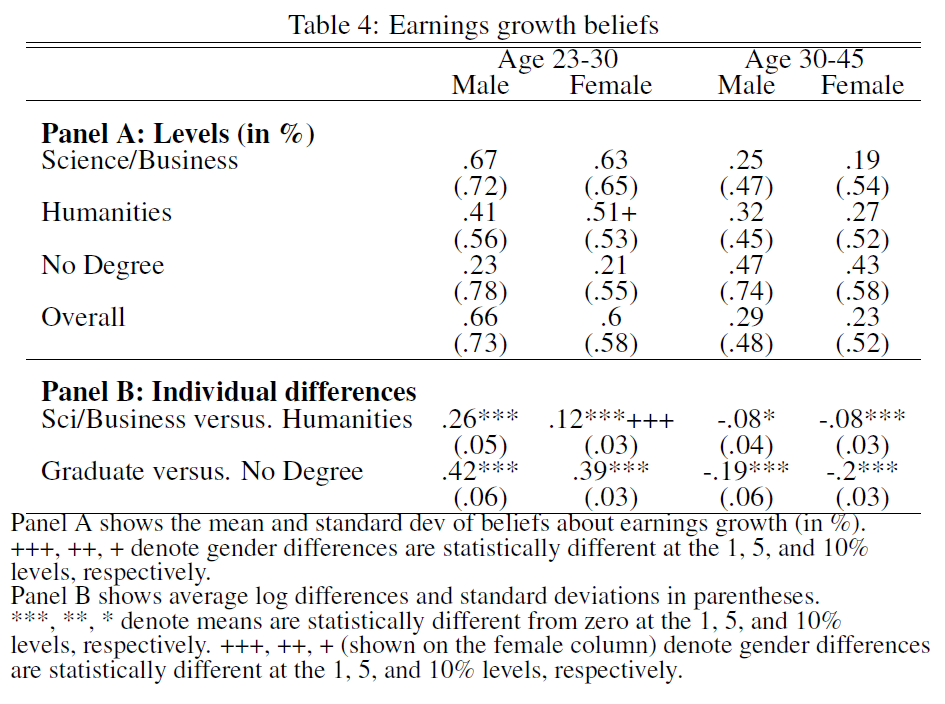
\includegraphics[scale=0.35]{Graphs/Table 4 Earnings Growth Belief.png}
\end{frame}

% Earnings Beliefs: Earnings Uncertainty
\begin{frame}{Earnings Uncertainty}
    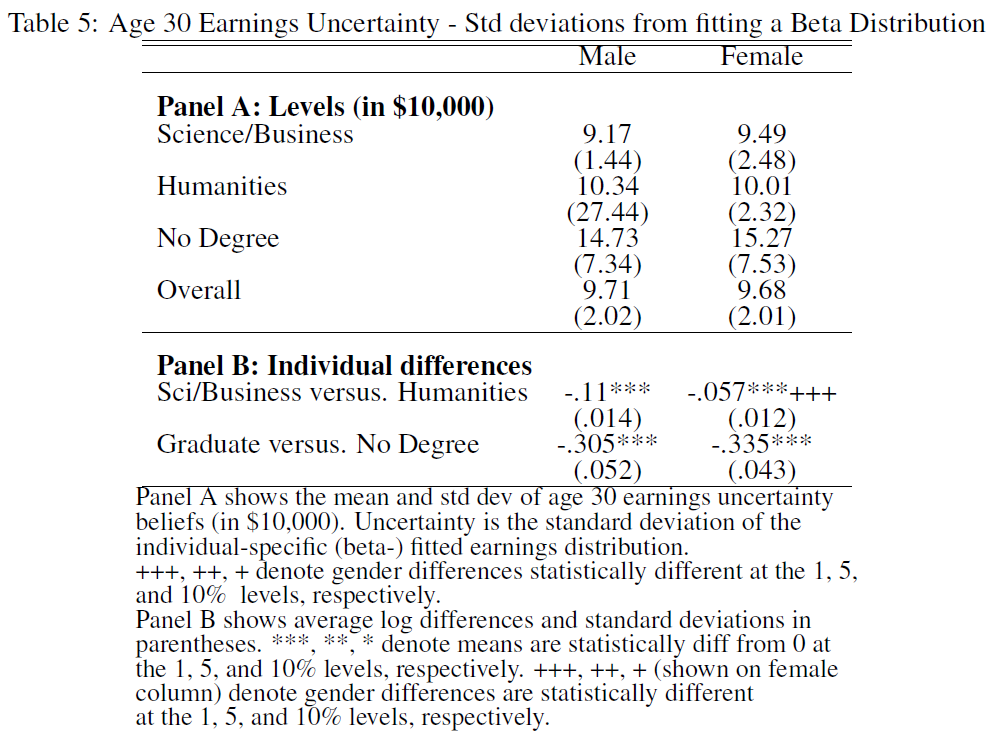
\includegraphics[scale=0.35]{Graphs/Table 5 Age 30 Earnings Uncertainty.png}
\end{frame}

% Beliefs about Marriage
\begin{frame}{Beliefs about Marriage}
    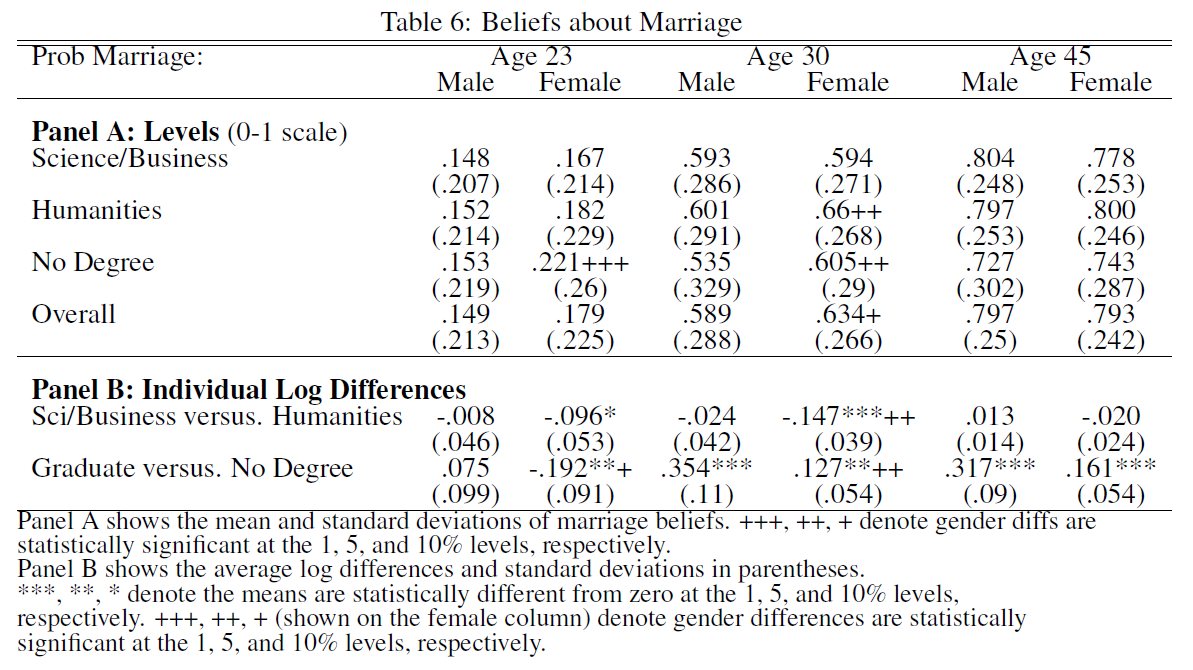
\includegraphics[scale=0.35]{Graphs/Table 6 Beliefs about Marriage.png}
\end{frame}

% Beliefs about Potential Spousal Earnings
\begin{frame}{Beliefs about Potential Spousal Earnings}
    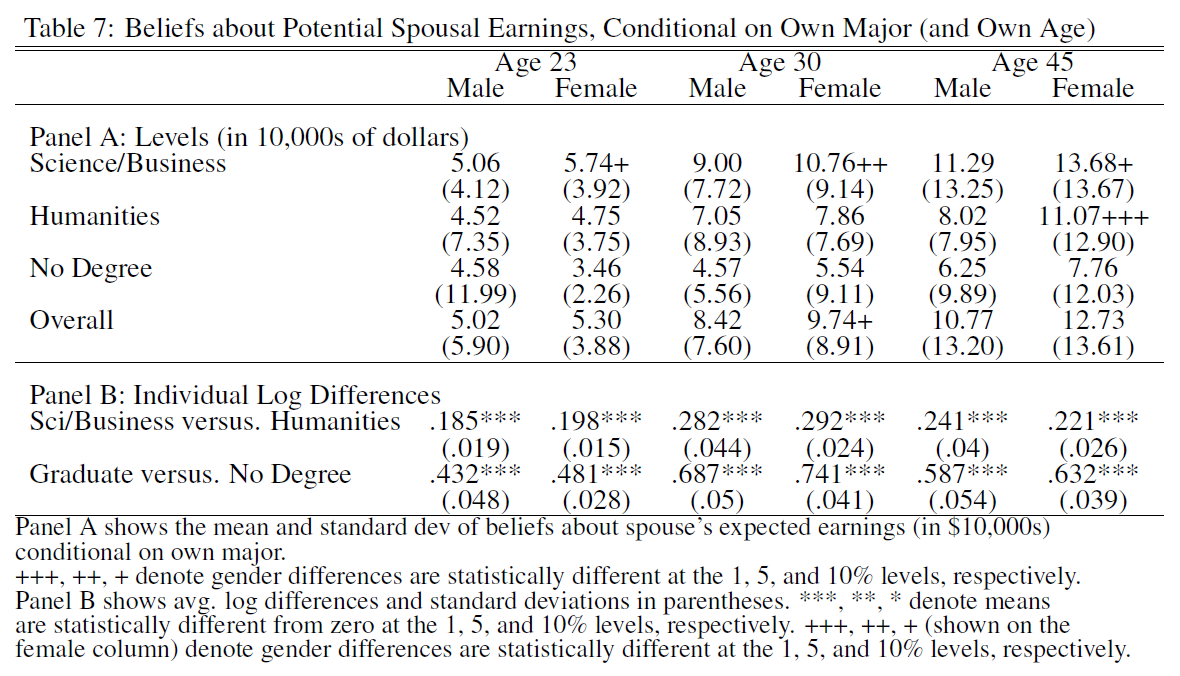
\includegraphics[scale=0.35]{Graphs/Table 7 Beliefs about Potential Spousal Earnings.png}
\end{frame}

\end{document}